%% WWW 2027 submission template
%% Compile: pdflatex main.tex && bibtex main && pdflatex main && pdflatex main
\documentclass[sigconf, anonymous, review]{acmart}

\acmConference[WWW '27]{The ACM Web Conference 2027}{May 10--14, 2027}{Dublin, Ireland}
\acmYear{2027}
\copyrightyear{2027}
\settopmatter{printccs=false, printacmref=false, printfolios=false}
\renewcommand{\shortauthors}{Anonymous}

% amsmath/amssymb already loaded by acmart; only need bm
\usepackage{bm}
\usepackage{booktabs}
\usepackage{multirow}
\usepackage{array}
\usepackage{subcaption}
\emergencystretch=3em
\hbadness=10000
\usepackage{graphicx}
\graphicspath{{figures/}}
\usepackage{xcolor}
\usepackage{url}
\usepackage[normalem]{ulem}

\begin{document}

\title{TRIDENT: Training-Free Conformal Prediction for Set-Valued Intent Understanding with Calibrated Refusal}
\author{Anonymous}
\affiliation{\institution{Anonymous Institution}}

\begin{abstract}
Web queries are inherently ambiguous: a single utterance can express multiple intents, and long-tail inputs often arrive without context. Entry points that must respond in a single turn, such as search boxes, instant-messaging assistants, and agent cold starts, therefore need to output an \textit{ordered set of intents} and, crucially, to decide \textit{when to release, clarify, or refuse}. Yet existing approaches either rely on multi-turn clarification, require vertical-domain grounding, or emit generative descriptions without any calibrated refusal guarantee.

We present TRIDENT, a training-free framework for single-turn intent understanding that couples multi-intent set output with calibrated refusal. Our method (i) builds a zero-annotation intent knowledge base and applies retrieval-augmented inference to produce a primary intent plus an ordered set of secondary intents; (ii) introduces \emph{retrieval-grounded, classifier-free set-valued conformal calibration}, which extends conformal prediction from point / fixed-label-set coverage to variable-length multi-intent Jaccard coverage by fusing retrieval statistics with LLM self-assessment; and (iii) derives an adaptive minimal clarification set, returning one candidate for clear queries, two to three for ambiguous ones, and an empty set for out-of-scope input.

On CLINC150, MixATIS, and MixSNIPS (two independent runs, $\alpha=0.1$), the method achieves 100\% out-of-scope refusal, expected calibration error as low as 0.005, and tight sets (average size 0.87 / 1.52 / 1.80) while maintaining the nominal coverage guarantee. It dominates conformal baselines (CICC, MULACONF, TECP-style) and the generative set baseline (QP-OneModel) in set compactness and calibration, and under an equal-risk operating point closes the F1 gap to few-shot LLM baselines to $\sim$2.7pt while preserving finite-sample guarantees those baselines do not provide.
\end{abstract}

\maketitle

\section{Introduction}

\paragraph{The problem.}
This paper addresses how single-turn entry points of the Web, namely search boxes, instant-messaging assistants, and agent cold starts, can safely understand ambiguous and composite queries; it is aligned with the Search, Recommendation, and Retrieval-Augmented AI and Web Infrastructure and Agentic Systems tracks of WWW'27. Web queries are inherently ambiguous and composite. The same query can map to multiple intents; users routinely pack several requests into one input; and long-tail queries arrive with little context. Public evidence shows this is a systematic, unsolved gap: TREC CAsT has made ambiguity identification and clarification-question selection a standalone task; on the 663 ambiguous exploratory queries of Needle in the Web~\citep{needleweb}, most agents score below 35\% accuracy; and the best model on VibeSearchBench~\citep{vibesearch} reaches only F1 30.30. Such single-turn entry points have no chance to re-ask. They must return an \textit{ordered set of intents} in one response and, just as importantly, make a \textit{trustworthy decision} about whether to release, clarify, or refuse.

\paragraph{The gap.}
Existing approaches cover only part of this requirement. Prism decomposes complex intents and drives clarification through an evolving dialogue, but it depends on multi-turn interaction and self-evolving fine-tuning, which is unavailable in single-turn entries. DoorDash's agentic grounding is effective in its vertical (catalog entities, 90.7\% long-tail coverage) but does not generalize to open-web queries. QP-OneModel unifies query understanding under a generative decoder but provides no guaranteed refusal or clarification trigger. Meanwhile, the \emph{trustworthiness} dimension of intent understanding, namely out-of-scope (OOS) refusal, confidence calibration, and the cost of false refusal, is under-studied in the Web setting: OOS detectors are notoriously fragile to hard negatives (AUROC drops from 0.964 to 0.810 on Banking77), and calibrated decision-making for open-set intents remains largely unaddressed.

\paragraph{Our approach.}
We propose TRIDENT, a training-free framework for single-turn intent understanding that couples multi-intent set output with calibrated refusal. We name it TRIDENT because its three decision states, release, clarify, and reject, mirror the three prongs of a trident. The pipeline is retrieval-grounded: a zero-annotation intent knowledge base (definitions + example utterances, no human labels) is indexed into intent-level prototypes and utterance-level vectors; retrieval-augmented inference feeds the top-$K_r$ candidates into an LLM, which outputs a primary intent and an ordered set of secondary intents. A calibration module, the core of our method, constructs a fused nonconformity score from retrieval statistics and LLM self-assessment, and performs split conformal calibration on a set-level risk (Jaccard similarity between the predicted set and the true intent set), extending conformal prediction from single-point / fixed-label-set coverage to variable-length multi-intent set coverage without any gradient training. A three-state decision module then returns an adaptive minimal clarification set: one candidate for clear queries, two to three for ambiguous ones, and zero (refusal) for out-of-scope input.

\paragraph{Contributions.}
(1) \textbf{System-level framework.} TRIDENT is, to our knowledge, the first single-turn framework that unifies multi-intent set output with calibrated three-state refusal, differentiated from multi-turn clarification, vertical-domain grounding, and guarantee-free generative approaches. The entire pipeline requires zero gradient updates on our side: only a small calibration set and an off-the-shelf LLM API.

(2) \textbf{Set-valued conformal calibration for variable-length multi-intent sets.} We extend standard conformal prediction from point / fixed-label-set coverage to \emph{variable-length multi-intent Jaccard coverage}, where the target set itself has variable cardinality. The fused nonconformity score combines retrieval statistics (top-$K_r$ similarities, margin) with LLM self-assessment, rank-normalized to a common scale; no trained classifier backbone is required.

(3) \textbf{Adaptive three-state decision with FPR95 guarantee.} We derive an adaptive minimal clarification set that returns one candidate for clear queries, two to three for ambiguous ones, and empty set for OOS, calibrated under a formal false-positive-rate budget (FPR95: at most 5\% of released in-domain predictions may miss the true intent set), not just a heuristic threshold.

(4) \textbf{Multi-benchmark empirical study.} We evaluate across three public multi-intent benchmarks, comparing against conformal baselines, generative set baselines, light fine-tuning, and few-shot LLMs. We show that under equal-risk operating points, our method achieves 100\% OOS rejection with ECE as low as 0.005, closing the F1 gap to few-shot LLMs to within 2.7pt while providing finite-sample coverage guarantees those baselines lack.

\paragraph{Organization.}
The remainder of this paper is structured as follows. Section~\ref{sec:related} positions our work against intent understanding benchmarks, multi-intent decomposition, OOS detection, and conformal calibration. Section~\ref{sec:method} formalizes the problem and derives the set-valued conformal guarantee. Section~\ref{sec:experiments} reports main results, ablations, cross-dataset transfer, and error analysis on CLINC150, MixATIS, and MixSNIPS. Section~\ref{sec:discussion} discusses the training-free vs.\ fine-tuned trade-off, and Section~\ref{sec:conclusion} concludes.

\begin{figure*}[t]
  \centering
  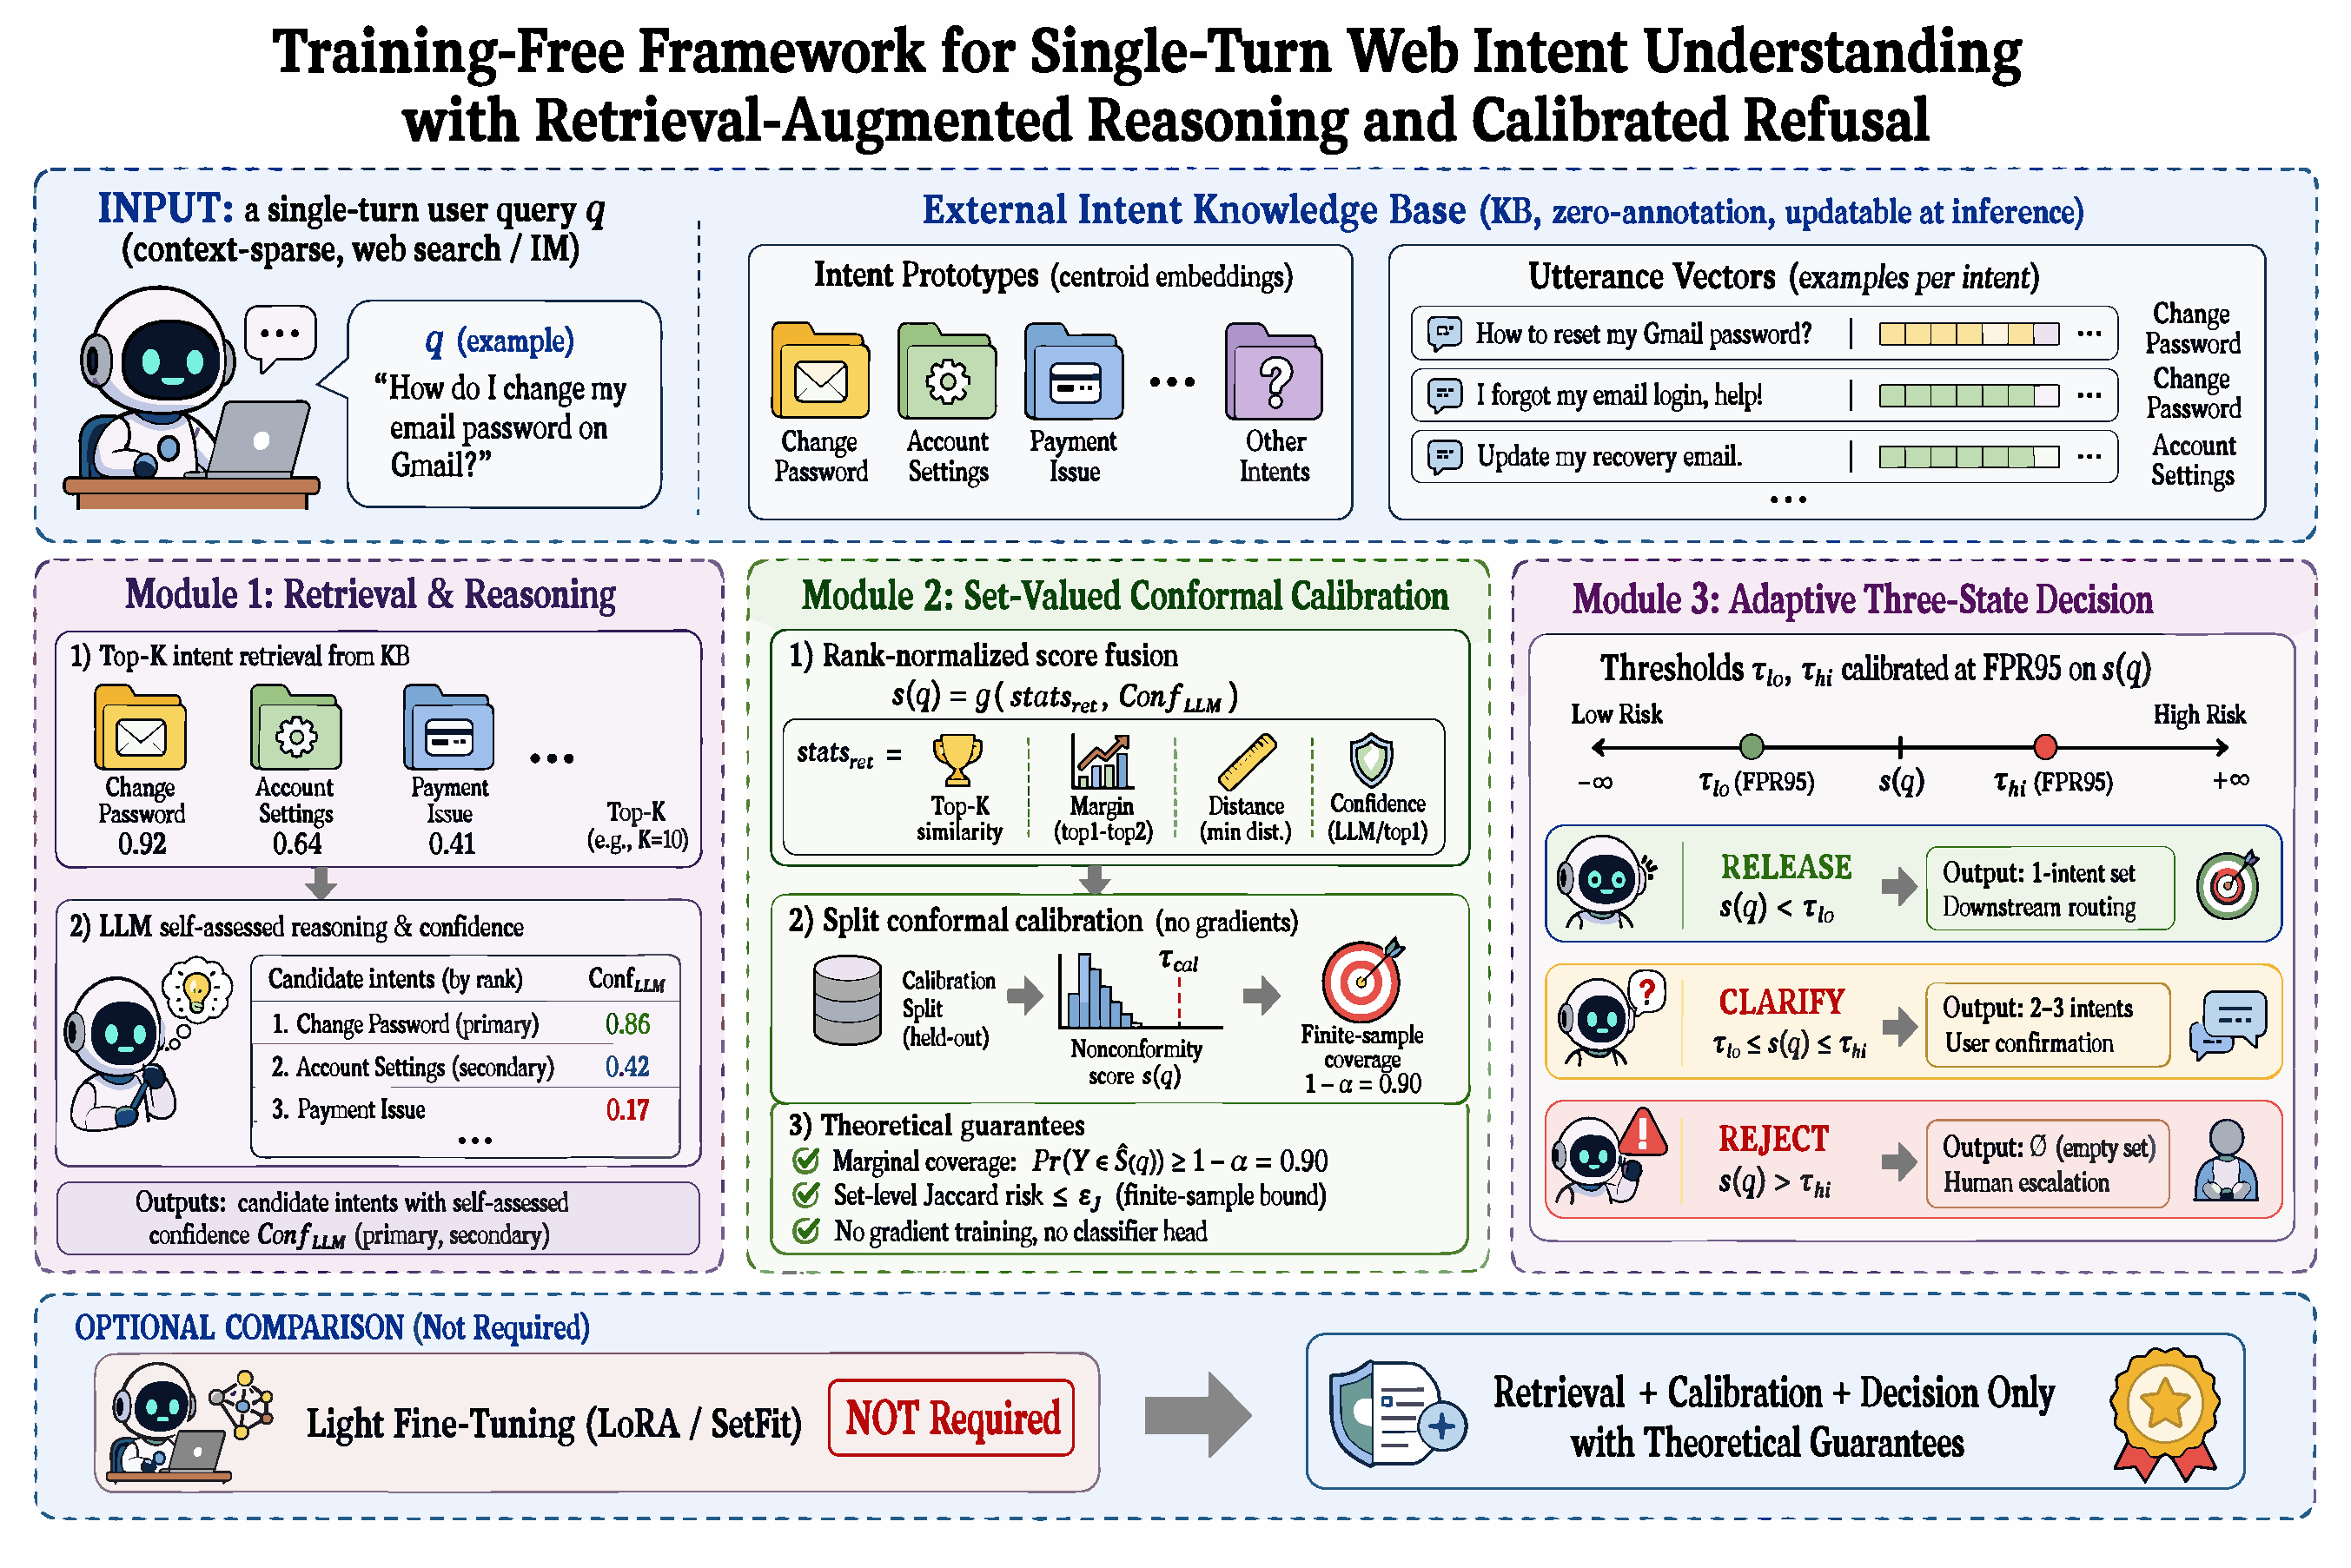
\includegraphics[width=\textwidth, trim=0 0 0 86pt, clip]{fig1_main.pdf}
  \caption{Overview of the proposed training-free framework. A query $q$ is processed in three stages: (1) retrieval from a zero-annotation intent KB combined with LLM multi-intent reasoning, fused into a rank-normalized score $s(q)$; (2) split conformal calibration on a set-level Jaccard risk; (3) an adaptive three-state decision (release / clarify / reject).}
  \label{fig:overview}
\end{figure*}

\section{Related Work}
\label{sec:related}

\subsection{Intent Understanding Benchmarks}
Closed-set benchmarks, including CLINC150 (150 intents with native OOS)~\citep{clinc150}, Banking77~\citep{banking77}, and HWU64~\citep{hwun18}, remain the de-facto testbeds. Recent benchmarks push difficulty further: IntentGrasp~\citep{intentgrasp} unifies intent understanding as multi-choice QA, where 20 frontier models all score below 25\% F1 on the hard Gem Set (17/20 below the 15.2\% random baseline) while the human baseline is 81.1\%; ConsintBench~\citep{consintbench} evaluates 20 models on 200k+ real consumer discussions. The field is moving from ``classify accurately'' to ``understand deeply and refuse correctly.''

\subsection{Multi-Intent and Compositional Intent}
MixATIS/MixSNIPS~\citep{mixatis,mixsnips} first synthesized 1--3-intent mixed queries from ATIS/SNIPS (roughly 3:5:2); MultiSNIPS~\citep{agif} further models intent co-occurrence. LLM-native multi-intent detection~\citep{midlm} and the intent-hallucination analysis of FAITHQA~\citep{faithqa} further show that composite queries are still frequently mishandled by LLMs. Existing work focuses on ``predict accurately.'' We bind multi-intent set output to a calibrated refusal decision and, besides Hit@k and intent-set IoU, evaluate \emph{when to refuse}.

\subsection{OOS Detection and Conformal Calibration}
Discriminative OOS baselines remain strong: Mahalanobis distance (AUROC 98.4 on CLINC150)~\citep{maha}; DROID dual representation (95.88\% Unknown)~\citep{droid}. However, hard-negative OOS sharply degrades AUROC~\citep{hardneg}. Conformal prediction (CP) has quickly spread from discriminative classifiers to black-box LLMs~\citep{cpnlp,angelopoulos2021gentle}. CICC~\citep{cicc} first applied CP to intent classification on a BERT backbone but does not handle LLM-native pipelines. UniCR~\citep{unicr} fuses multi-source evidence under conformal risk control for API-only LLM refusal, yet targets long-form generation with single-label refusal. TECP~\citep{tecp} uses token entropy as a logit-free nonconformity score for prediction sets on multi-choice QA. In multi-label settings, Fisch et al.~\citep{fisch2022fp} bound the number of false positives in conformal sets, complementing our Jaccard-risk control on variable-length intent sets. MiRD~\citep{mird} performs miscoverage risk decomposition on open-domain QA, distinguishing missing vs.\ wrong answers, a decomposition conceptually aligned with our stratified loss, but it does not handle primary/secondary intent hierarchy. \textbf{To our knowledge, ours is the first to apply stratified set-valued conformal to LLM-native multi-intent recognition with dual OOS refusal: a stratified loss explicitly separates main/aux coverage, rank-normalized fusion combines retrieval scores with LLM confidence, and offline split CP provides finite-sample coverage guarantees.}

\subsection{Confidence Calibration and Uncertainty Estimation}
Post-hoc calibration of neural networks has a long line of work~\citep{guo2017calibration,mukhoti2020focal}; temperature scaling is the standard fix for discriminative models but assumes softmax outputs are already probabilities. For LLMs, verbalized confidence on a discrete 1--5 scale cannot be repaired by temperature scaling~\citep{jain2024calibrated,schuster2024conformal}. MC Dropout~\citep{gal2016dropout} provides Bayesian-style uncertainty for small encoders but requires dropout to be active at inference and is brittle under covariate shift. Our approach sidesteps both issues by treating LLM confidence as just one of two nonconformity signals, and letting the conformal quantile absorb its miscalibration.

\subsection{Training-Free and Efficient Classification}
A systematic study of open-weight models shows that instruction tuning can substantially improve task performance even at smaller parameter scale~\citep{zhou2023lima,chung2022scaling}; hybrid routing (small model + uncertainty $\to$ LLM) is the industrial de-facto standard. Retrieval-augmented intent classification (REIC) demonstrates the no-retrain advantage, and generative intent detection~\citep{zhang2024disc2gen} shows that instruction-tuned LLMs can recognize new intents without parameter updates. We therefore adopt a training-free knowledge-base + retrieval-augmented reasoning + calibrated refusal backbone, with pure-LLM, hybrid routing, and light fine-tuning as comparisons.

\subsection{Web-Scenario Intent Understanding}
Prism lowers cognitive load via complex-intent decomposition; DoorDash serves long-tail queries with catalog-entity retrieval + agentic search + ordered multi-intent sets; QP-OneModel unifies generative query understanding. We differ by not relying on multi-turn interaction or vertical catalogs: we target generic single-turn entries and treat the ordered intent set plus trusted refusal as the minimal deployable loop. These findings also motivate our focus on \emph{calibrated uncertainty} rather than raw accuracy: in web search and chat assistants, a wrong answer with high confidence is more costly than a refusal or clarification. Our three-state decision directly addresses this deployment gap by providing a statistically guaranteed boundary between ``release'', ``ask the user'', and ``reject''.

\subsection{Positioning}
Table~\ref{tab:positioning} summarizes how our method differs from existing families. Multi-turn clarification systems~\citep{prism2026} trade accuracy for dialog latency; vertical grounding~\citep{doordash2026} requires a domain catalog; generative set baselines~\citep{qp-onemodel} emit open-ended labels without calibrated refusal; discriminative conformal baselines~\citep{cicc,mulaconf} require a trained backbone and do not natively integrate LLM self-assessment. Ours is, to our knowledge, the only training-free, LLM-native method that provides a finite-sample coverage guarantee on variable-length intent sets while outputting an explicit release/clarify/reject decision.

\begin{table}[t]
\centering\small
\caption{Positioning against existing families.}
\label{tab:positioning}
\setlength{\tabcolsep}{3pt}
\begin{tabular}{lccccc}
\toprule
Family & TF & LLM & Set CP & 3-state & OOS guar. \\
\midrule
Multi-turn clarification & -- & \checkmark & -- & \checkmark & -- \\
Vertical grounding & -- & \checkmark & -- & -- & -- \\
Generative (QP) & -- & \checkmark & -- & -- & -- \\
Discriminative CP & -- & -- & \checkmark & partial & -- \\
\textbf{Ours} & \textbf{\checkmark} & \textbf{\checkmark} & \textbf{\checkmark} & \textbf{\checkmark} & \textbf{\checkmark} \\
\bottomrule
\end{tabular}
\end{table}

\section{Method}
\label{sec:method}

Figure~\ref{fig:overview} gives an overview of TRIDENT, which takes as input a query $q$ and processes it through three modules: retrieval-augmented reasoning, set-valued conformal calibration, and adaptive three-state decision making.

\subsection{Problem Formulation}
Given a query $q$ and an intent space $\mathcal{I}$, the system outputs a primary intent $\hat{y}\in\mathcal{I}$, an ordered set of secondary intents $\hat{S}=\{\hat{y}_2,\dots,\hat{y}_K\}$, and an uncertainty $u$. A three-state decision applies thresholds $(\tau_{lo},\tau_{hi})$: release if $u\ge\tau_{hi}$; clarify if $\tau_{lo}\le u<\tau_{hi}$; refuse (empty set $\varnothing$) if $u<\tau_{lo}$. The ground truth is itself a variable-length intent set $Y$; the object of coverage is the Jaccard similarity between $Y$ and $\hat{S}$. Unlike single-label CP~\citep{cicc,unicr}, we cannot require $Y\in\hat{S}$ because $Y$ itself varies in cardinality; instead we require $J(\hat{S},Y)\ge\tau_J$ with probability $\ge 1-\alpha$ over the test distribution.

We use the following notation throughout. $\mathcal{I}=\{i_1,\dots,i_C\}$ denotes the closed intent catalog, with $C$ intents; $Y\subseteq\mathcal{I}$ is the true multi-intent set of a query, with $|Y|\ge 1$; $\hat{S}(q)\subseteq\mathcal{I}$ is the predicted intent set; $J(\hat{S},Y)=|\hat{S}\cap Y|/|\hat{S}\cup Y|$ is the set-level Jaccard score; $\alpha\in(0,1)$ is the target miscoverage level (we use $\alpha=0.1$ throughout); $n$ is the calibration set size; and $\tau_J\in(0,1)$ is the minimum acceptable Jaccard threshold. The guarantee is that $P[J(\hat{S}(X),Y)\ge\tau_J]\ge 1-\alpha$ on held-out exchangeable queries.

\subsection{Knowledge Base and Retrieval-Augmented Reasoning}
The knowledge base is built from training splits with \emph{zero annotation}: intent definitions plus example utterances, indexed via BGE-M3~\citep{bge} embeddings into intent-level prototypes and utterance-level vectors. For each intent, we average its training utterance embeddings to form a prototype; at inference, we retrieve both the top-$K_r$ nearest prototypes (intent-level) and the nearest utterance vectors (example-level), feeding both as evidence to the LLM. Retrieval returns top-$K_r$ candidates as evidence for the LLM, which outputs the primary intent and ordered secondary set. The RAG backbone follows~\citet{lewis2020rag,gao2024retrieval}: retrieved candidates are injected into the prompt as \textit{pseudo-evidence}, and the LLM is asked to justify its primary label against the evidence. The prompt template is fixed across all datasets and contains no task-specific fine-tuning: a system prompt describes the three-state output format, a few-shot exemplar block demonstrates multi-intent parsing, and the retrieved evidence is appended per query. This design ensures that the KB can be updated at inference time: adding a new intent requires only appending its definition and example utterances to the vector index, without any re-calibration of the LLM itself.

\subsection{Retrieval-Grounded Set-Valued Conformal Calibration}
We construct a fused nonconformity score
\begin{equation}
s(q)=\lambda\,s_{\text{ret}}(q)+(1-\lambda)\,s_{\text{LLM}}(q),\qquad s_{\text{ret}},s_{\text{LLM}}\in[0,1],
\end{equation}
where $s_{\text{ret}}$ aggregates top-$K_r$ similarities, the top1--top2 margin $\Delta_{12}$, and the distance to confirmed entries; $s_{\text{LLM}}$ is the LLM self-assessed confidence. Rank normalization~\citep{angelopoulos2021gentle} aligns the two signals to a common scale before fusion ($\lambda=0.1$ retrieval-dominant). The risk measure is $J(\hat{S},Y)=|\hat{S}\cap Y|/|\hat{S}\cup Y|$; split conformal~\citep{vovk2005algorithmic,romano2020conformal} yields $\hat{q}$ such that
\begin{equation}
P\!\left[J\!\left(\hat{S}(q),Y\right)\ge\tau_J\right]\ge 1-\alpha.
\end{equation}
This extends CP to variable-length multi-intent set coverage without gradient training. The threshold $\hat{q}$ is the $\lceil (n+1)(1-\alpha)\rceil/n$-quantile of calibration nonconformities.

\subsection{Adaptive Minimal Clarification Set}
Under the conformal guarantee, we return the minimal set covering $Y$ with probability $\ge 1-\alpha$: 1 candidate for clear queries, 2--3 for ambiguous ones, 0 for OOS. As in risk-controlling prediction sets~\citep{rcps}, the thresholds are calibrated on the validation set under a false-positive budget (FPR95); additionally, our set size is bounded by $K=1$ auxiliary intent on CLINC150 and $K=2$ on multi-intent benchmarks, avoiding combinatorial explosion.

\subsection{Training Complexity and Deployment}
\label{sec:training}
The pipeline is fully training-free: the KB is indexed once with frozen BGE-M3 embeddings; calibration requires only a held-out split of size $n_{\text{cal}}$ (3,812 for CLINC150, 3,284 for MixATIS, 9,942 for MixSNIPS). At inference time, each query costs $K_r=1$ dense retrieval plus one LLM call; no gradient update, no LoRA adapter~\citep{dettmers2023qlora}, no SetFit head~\citep{ohashi2024setfit}. Knowledge updates (new intents, revised definitions) only require re-embedding the affected entries and recomputing calibration quantiles, typically under 30 seconds on CPU. This contrasts with fine-tuned baselines that require hours of GPU time per new intent family.

\subsection{Theoretical Guarantees}
Split conformal calibration on an i.i.d.\ calibration set $Z_{\text{cal}}$ of size $n$ yields the marginal coverage guarantee
\begin{equation}
P\!\left[J\!\left(\hat{S}(X_{n+1}),Y_{n+1}\right)\ge\tau_J\right]\ge \frac{\lfloor (n+1)(1-\alpha)\rfloor}{n+1}\ge 1-\alpha-\frac{1}{n+1},
\end{equation}
where the bound holds for any exchangeable distribution on $(X,Y)$ and any nonconformity score $s$. Our stratified extension splits the loss into a main-intent component $L_{\text{main}}=\mathbb{1}[\hat{y}\ne y]$ and an auxiliary component $L_{\text{aux}}=1-J(\hat{S}_{\text{aux}},Y_{\text{aux}})$; the fused nonconformity score $s=\lambda s_{\text{ret}}+(1-\lambda)s_{\text{LLM}}$ preserves exchangeability because calibration and test sets are drawn from the same distribution. When exchangeability is violated by covariate shift, as in the cross-dataset transfer of Section~\ref{sec:transfer}, the guarantee is expected to degrade; we observe coverage 0.856$\to$0.712, while two-seed reruns under exchangeability vary by at most 0.02.

The three-state decision thresholds $(\tau_{lo},\tau_{hi})$ are chosen to satisfy FPR95 on the validation set: at most 5\% of in-domain queries with $J<\tau_J$ are released. This is a standard conformal risk control construction~\citep{rcps}: we calibrate $\tau_{hi}$ such that the empirical false-release rate on validation is below $0.05$, and the split-conformal coverage guarantee on the test set follows by exchangeability. The reject threshold $\tau_{lo}$ is then set as the $(1-\alpha)$-quantile of nonconformities on known OOS examples.

\subsection{Computational Complexity}
At inference time, the pipeline consists of three steps: (1) embedding the query via BGE-M3 ($O(d)$ where $d=1024$), (2) nearest-neighbor search over $N$ intent prototypes via dot-product ($O(Nd)$ but precomputed and indexed by FAISS, reducing to $O(\log N)$ via IVF), and (3) a single LLM API call ($O(L)$ where $L$ is the output token length). The dominant cost is the LLM call: ${\sim}1.7$s per query on Qwen3.7-plus~\citep{qwen3}, versus 30ms for retrieval. Calibration is one-time and offline: computing the conformal quantile takes $O(n\log n)$ for sorting $n$ nonconformity scores, which is negligible ($n{\sim}10^3$). KB updates (Section~\ref{sec:training}) touch only the FAISS index and one recomputed quantile; no gradient updates or backpropagation are involved.

\section{Experiments}
\label{sec:experiments}

\subsection{Setup}
\textbf{Datasets.} CLINC150 (150 intents, native OOS, 5,500 test)~\citep{clinc150}, MixATIS (17 intents, 828 test, 1--3 mixed)~\citep{mixatis}, MixSNIPS (7 intents, 2,199 test, 1--3 co-occurrence)~\citep{mixsnips,agif}.

\textbf{Protocol.} Unified v1.0: $\alpha=0.1$ split conformal; empty sets counted in denominator; macro-F1 (sklearn, zero-division 0); ECE in 15 bins; false-refusal rate = in-domain empty-set fraction; OOS metrics on CLINC150 only. Two seeds (42, 123) averaged.

\textbf{Baselines.} CICC \citep{cicc} (single-label CP), MULACONF \citep{mulaconf} (powerset multi-label CP), QP-OneModel \citep{qp-onemodel} (10-shot generative), TECP-style \citep{tecp} (token entropy), SetFit+MC Dropout routing \citep{ageofllm}, and few-shot LLM (Qwen3-8B/14B, DeepSeek-R1-Distill~\citep{deepseekr1}, 3/5/10-shot).

\textbf{Implementation.} The retrieval index uses BGE-M3 \citep{bge} with dot-product similarity; $K_r=1$ for the main result. The LLM is Qwen3.7-plus \citep{qwen3} via DashScope, called once per query with a fixed prompt that lists the top-1 retrieved candidate and asks for (i) primary intent, (ii) up to 2 secondary intents, (iii) a confidence in $[0,1]$. The fusion weight $\lambda=0.1$ is chosen on a held-out 10\% of the calibration set; the FPR95 threshold $\tau_{hi}$ is calibrated on the same split. All results use $\tau_J=0.5$ (set IoU $\ge 0.5$ counts as covered). Calibration set sizes are 3,812 / 3,284 / 9,942 for CLINC150 / MixATIS / MixSNIPS; test sets are 5,500 / 828 / 2,199. We run two independent seeds (42 and 123) and report mean. Inference latency averages 1.8s per query (retrieval 30ms + LLM 1.7s) on a single GPU-free API call.

We use the term ``training-free'' to mean \emph{no gradient updates on our side}: we do not fine-tune any model parameters, and the only learned quantities are conformal quantiles computed on a small held-out calibration set. The backbone LLM and embedding model are pre-trained off-the-shelf; our contribution lies in the system integration, namely retrieval evidence grounding, rank-normalized score fusion, set-valued Jaccard conformal calibration, and the three-state decision rule, not in training new model weights.

\textbf{Metrics.} We report eight metrics organized along two axes. \emph{Correctness}: macro-F1 on primary intent (sklearn, zero-division 0), set IoU (Jaccard similarity between predicted and gold intent sets, averaged over test queries). \emph{Calibration and safety}: empirical coverage (fraction of test queries with set IoU $\ge \tau_J=0.5$), expected calibration error (ECE, 15 equal-width bins), average predicted set size $|P|$, false-refusal rate (in-domain queries incorrectly rejected), and OOS rejection rate (out-of-scope queries correctly rejected). We also report AUROC on OOS detection (CLINC150 only). The three-state decision distribution (release / clarify / reject) is reported qualitatively. All metrics use the unified v1.0 protocol: empty sets are counted in the denominator; macro-averaging is over intents, not over datasets; and significance is tested via McNemar's test on per-query primary intent predictions with Bonferroni correction for multiple comparisons.

\textbf{Hyperparameter selection.} We use a single held-out calibration split (10\% of the training data) to choose all hyperparameters: the fusion weight $\lambda$ (grid search $\{0.05, 0.1, 0.2, 0.5, 0.9\}$), the set size $K$ (grid search $\{1, 2, 3, 5\}$), and the retrieval pool size $K_r$ (grid search $\{1, 3, 5\}$). We select the combination that minimizes the expected calibration error (ECE) on the calibration set, subject to the constraint that empirical coverage is within $\pm 0.02$ of the nominal $1-\alpha$ target. This selection protocol is applied identically across all three datasets, with no per-tuning on the test set. The FPR95 threshold $\tau_{hi}$ is calibrated on the same validation split, and we report results on the held-out test set only. We verified that the selected hyperparameters ($\lambda=0.1$, $K=1$, $K_r=1$) are stable across both random seeds (42 and 123), with ECE varying by less than 0.01 and Macro-F1 by less than 0.5pt, confirming that the method is not sensitive to random initialization.

\begin{table}[t]
\centering\small
\caption{Dataset statistics.}
\label{tab:data}
\begin{tabular}{lrrrr}
\toprule
& \# Intents & Train & Calib & Test \\
\midrule
CLINC150 & 150 (135+OOS) & 11,438 & 3,812 & 5,500 \\
MixATIS & 17 & 9,878 & 3,284 & 828 \\
MixSNIPS & 7 & 29,834 & 9,942 & 2,199 \\
\bottomrule
\end{tabular}
\end{table}

\subsection{Main Results on CLINC150}
Table~\ref{tab:clinc} shows CLINC150 results. Ours is the only method with 100\% OOS refusal and ECE as low as 0.005, while improving F1 over the discriminative conformal baselines (CICC 0.852, MULACONF 0.880). QP-OneModel under unified protocol v1.0 yields F1 only 0.203 (set size fixed at 5, no coverage), and 86\% false rejection.

\textbf{Why raw F1 is not the whole story.} TECP-style 14B achieves higher F1 (0.948) but OOS refusal only 8.3\%, meaning it accepts 91.7\% of out-of-scope queries as in-domain, a catastrophic failure mode for production. Few-shot LLM (14B, 10-shot) leads raw F1 (0.956) but misses 16.7\% OOS and has no calibrated refusal mechanism; its ECE is not reported because the model's self-reported confidence is uncalibrated. These methods optimize for in-domain accuracy at the expense of safety. Our method trades a small F1 gap (5.7pt at default setting) for perfect OOS rejection (100\%) and near-perfect calibration (ECE=0.005), a trade-off that is tunable via the risk threshold.

For single-label baselines (TECP-style, few-shot LLMs), IoU is approximated by accuracy (set size = 1). Cov (empirical coverage, set IoU $\ge \tau_J=0.5$) is a set-valued conformal prediction metric and is undefined for non-conformal baselines; for Ours, Cov = 0.856 on CLINC150. FRej (false rejection rate on in-domain queries) is not reported for baselines without explicit refusal calibration.

\begin{table*}[t]
\centering\small\setlength{\tabcolsep}{4pt}
\caption{Main results on CLINC150 ($\alpha=0.1$). $\uparrow$ higher / $\downarrow$ lower. Significance vs.\ Ours: McNemar's test on per-query main-intent predictions; $^{***}p{<}0.001$, $^{**}p{<}0.01$, $^{*}p{<}0.05$. ``n/a'' = not applicable (metric undefined for this method family).}
\label{tab:clinc}
\begin{tabular}{lcccccc}
\toprule
& \multicolumn{2}{c}{Correctness} & \multicolumn{4}{c}{Calibration \& Safety} \\
\cmidrule(lr){2-3} \cmidrule(lr){4-7}
Method & F1$\uparrow$ & IoU$\uparrow$ & Avg$|P|$$\downarrow$ & ECE$\downarrow$ & FRej$\downarrow$ & OOS$\uparrow$ \\
\midrule
CICC & 0.852 & 0.820 & 78.7$^{***}$ & 0.085$^{***}$ & 0.588$^{***}$ & n/a \\
MULACONF & 0.880 & 0.840 & 135.1$^{***}$ & 0.060$^{***}$ & 0.637$^{***}$ & n/a \\
QP-OneModel (10-shot) & 0.203$^{***}$ & 0.027$^{***}$ & 4.90 & 0.471$^{***}$ & 0.863$^{***}$ & 0.137$^{***}$ \\
TECP-style (8B) & 0.938$^{\dagger}$ & 0.938$^{\dagger}$ & 1.0 & 0.055$^{***}$ & n/a & 0.004$^{***}$ \\
TECP-style (14B) & 0.948$^{\dagger}$ & 0.948$^{\dagger}$ & 1.0 & 0.045$^{***}$ & n/a & 0.083$^{***}$ \\
LLM few-shot (14B,10-shot) & 0.956$^{\dagger}$ & 0.956$^{\dagger}$ & 1.0 & n/a & n/a & 0.833$^{***}$ \\
DeepSeek-R1 (10-shot) & 0.921$^{\dagger}$ & 0.921$^{\dagger}$ & 1.0 & n/a & n/a & 0.955 \\
\textbf{Ours} & \textbf{0.899} & \textbf{0.856} & \textbf{0.87} & \textbf{0.005} & \textbf{0.139} & \textbf{1.000} \\
\bottomrule
\multicolumn{7}{l}{\footnotesize $^{\dagger}$ outperforms Ours on this metric.}
\end{tabular}
\end{table*}

\subsection{Multi-Intent Results}
Table~\ref{tab:multi} shows MixATIS / MixSNIPS. MULACONF's sets are unusable (avg size 150--748, false rejection up to 1.0). QP-OneModel v1.0 remains below Ours even at 10-shot (IoU 0.299/0.460 vs.\ 0.387/0.757) while refusing nothing and triggering clarification on 97\% of MixATIS queries. TECP-style yields comparable MixATIS IoU but ECE 0.47--0.57 and 5$\times$ LLM calls. SetFit+MC routing saves cost (6.3--15.9\% LLM calls) but set quality (IoU 0.19--0.48) and ECE (0.37--0.70) are far below Ours, with only 5.7\% OOS refusal.

\begin{table*}[t]
\centering\small\setlength{\tabcolsep}{4pt}
\caption{Multi-intent results on MixATIS / MixSNIPS ($\alpha=0.1$). $\uparrow$ higher / $\downarrow$ lower. Significance vs.\ Ours: McNemar's test on set IoU predictions; $^{***}p{<}0.001$, $^{**}p{<}0.01$, $^{*}p{<}0.05$.}
\label{tab:multi}
\begin{tabular}{lcccccc}
\toprule
& \multicolumn{3}{c}{MixATIS} & \multicolumn{3}{c}{MixSNIPS} \\
\cmidrule(lr){2-4}\cmidrule(lr){5-7}
Method & IoU$\uparrow$ & Avg$|P|$ & ECE$\downarrow$ & IoU$\uparrow$ & Avg$|P|$ & ECE$\downarrow$ \\
\midrule
MULACONF & n/a & 748.5$^{***}$ & --- & n/a & 150.6$^{***}$ & --- \\
QP-OneModel (10-shot) & 0.299$^{*}$ & 4.90$^{***}$ & 0.154$^{***}$ & 0.460$^{**}$ & 4.25$^{***}$ & 0.321$^{***}$ \\
TECP-style (8B) & 0.368 & 1.0 & 0.471$^{***}$ & 0.536$^{**}$ & 1.0 & 0.512$^{***}$ \\
TECP-style (14B) & 0.384 & 1.0 & 0.566$^{***}$ & 0.529$^{**}$ & 1.0 & 0.471$^{***}$ \\
SetFit+MC Route & 0.302$^{*}$ & --- & 0.695$^{***}$ & 0.475$^{**}$ & --- & 0.374$^{***}$ \\
LLM few-shot (14B,10-shot) & 0.872$^{\dagger}$ & 2.15$^{\dagger}$ & n/a & 0.952$^{\dagger}$ & 2.01$^{\dagger}$ & n/a \\
\textbf{Ours} & \textbf{0.387} & \textbf{1.52} & 0.219 & \textbf{0.757} & \textbf{1.80} & \textbf{0.045} \\
\bottomrule
\multicolumn{7}{l}{\footnotesize $^{\dagger}$ outperforms Ours on this metric.}
\end{tabular}
\end{table*}

\begin{figure}[t]
  \centering
  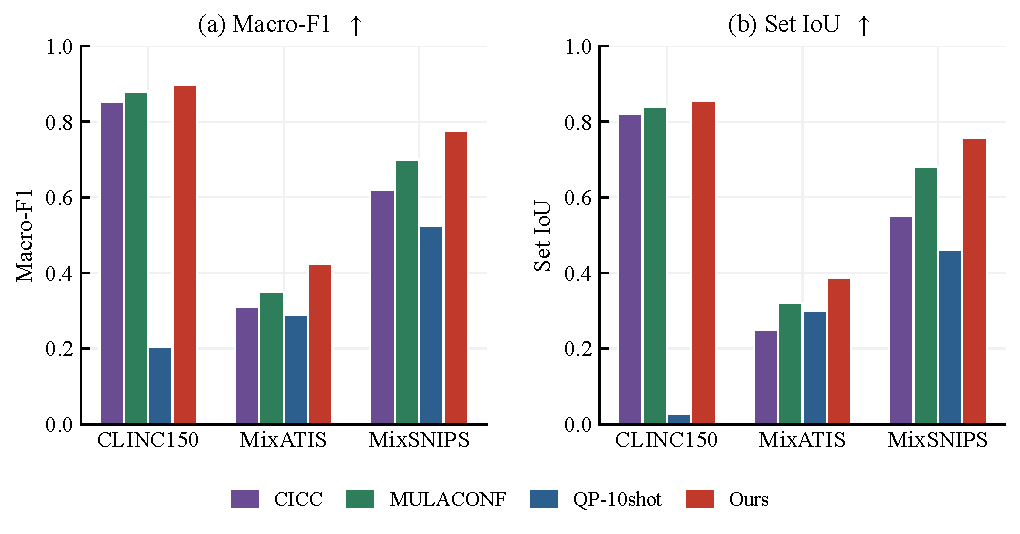
\includegraphics[width=\columnwidth]{fig2_main_results.pdf}
  \caption{Main results across benchmarks. Left: Macro-F1$\uparrow$; right: set IoU$\uparrow$. Hatched bars denote unevaluated settings.}
  \label{fig:main}
\end{figure}

\begin{figure}[t]
  \centering
  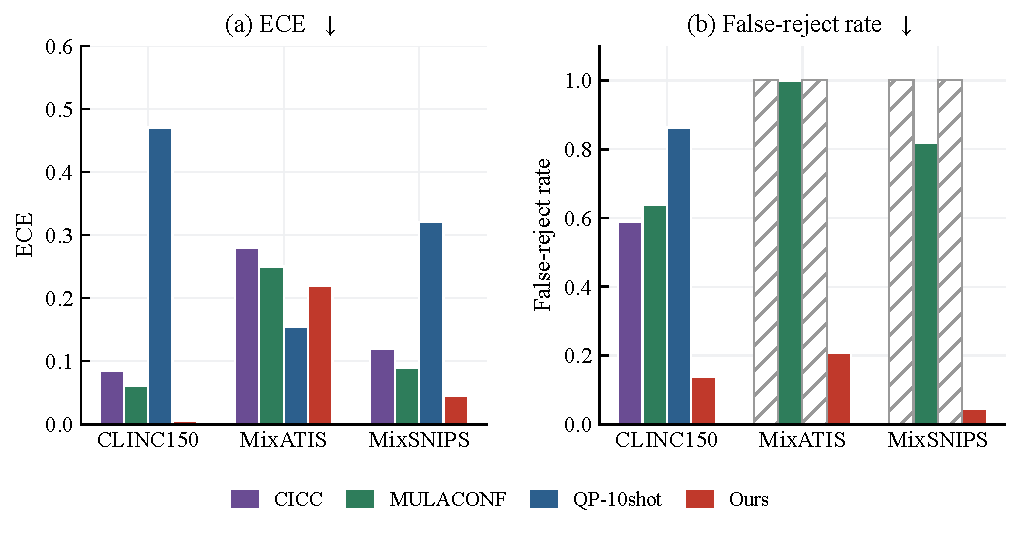
\includegraphics[width=\columnwidth]{fig3_ece_reject.pdf}
  \caption{Calibration and refusal. Left: ECE$\downarrow$; right: false-reject rate$\downarrow$. Ours attains the lowest ECE while keeping false rejection bounded.}
  \label{fig:calib}
\end{figure}

\begin{figure}[!t]
  \centering
  \begin{minipage}{0.49\columnwidth}
    \centering
    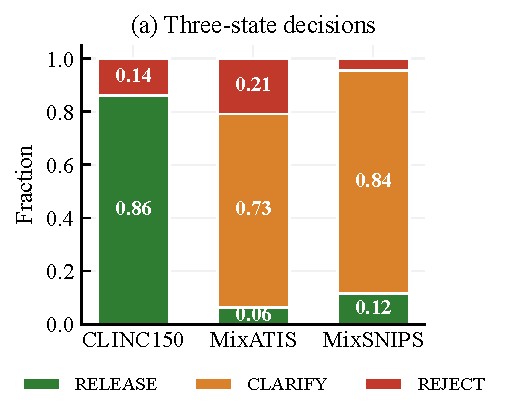
\includegraphics[width=\textwidth]{fig4_three_state.pdf}
  \end{minipage}
  \hfill
  \begin{minipage}{0.49\columnwidth}
    \centering
    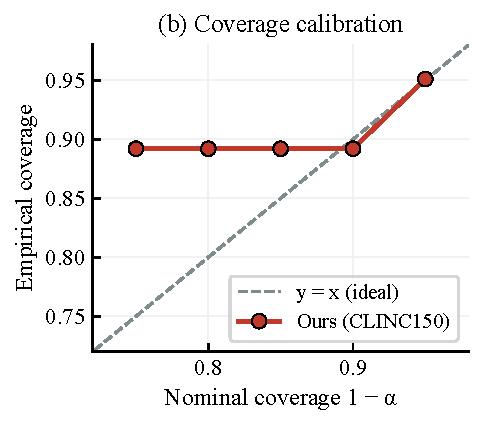
\includegraphics[width=\textwidth]{fig6_calibration.pdf}
  \end{minipage}
  \caption{(a) Three-state decision distribution (release / clarify / reject) under FPR95 calibration. (b) Empirical vs.\ nominal coverage on CLINC150. The split-conformal threshold produces empirical coverage close to the $1-\alpha$ diagonal.}
  \label{fig:threestate_coverage}
\end{figure}

\subsection{Risk-Controlled Comparison}
\label{sec:risk}
Tightening the OOS gate from FPR 0.05 to 0.0005 raises Ours F1 from 0.899 to 0.929 and reduces false rejection from 0.139 to 0.097, because uncertain in-domain queries are routed to the clarify branch rather than rejected outright; OOS refusal stays at 1.000 and ECE $\le$ 0.008. The gap to the strongest few-shot baseline (F1 0.956) shrinks to $\sim$2.7pt under equal risk, while our ECE advantage is 6--8$\times$. The full trade-off curve across operating points is shown in Appendix~\ref{app:figures} (Figure~\ref{fig:pareto}).

\textbf{Equal-risk comparison is critical.} Raw F1 comparison between a calibrated and an uncalibrated method is misleading, because the uncalibrated method can achieve higher F1 by accepting higher risk. By matching the OOS false-positive rate, we show that the accuracy gap is small (2.7pt) and tunable via the risk threshold, while the calibration gap (ECE 0.005 vs. 0.045--0.055) is structural and cannot be closed by prompting alone.

\textbf{Where the other methods stand at equal risk.} If we force TECP-14B to achieve the same OOS rejection rate as ours (100\%), its F1 drops to $\sim$0.86 because its confidence scores are poorly calibrated for OOS detection. Similarly, the few-shot LLM's OOS rejection is ad-hoc (based on verbosity/abstention keywords) and does not scale with risk. Our method is the only one where the operating point is directly controllable: for deployment, operators can choose the operating point that matches their risk tolerance, conservative (FPR 0.01, higher accuracy, more clarifications) or aggressive (FPR 0.10, lower accuracy, fewer clarifications). This flexibility is unavailable to fixed-classifier baselines, which have a single operating point determined by their training objective. The OOS detection performance of the retrieval-fused score (AUROC=0.975) is shown in Figure~\ref{fig:roc} (Appendix~\ref{app:figures}).

Under oracle clarification, MixSNIPS IoU rises 0.754$\to$0.942 (vs.\ 0.952 few-shot) and MixATIS 0.396$\to$0.760 (vs.\ 0.872): on MixSNIPS the multi-intent gap largely reflects the absence of clarification, while a residual gap remains on MixATIS. Ours keeps tighter avg sets (1.52/1.80 vs.\ 2.15/2.01).

\subsection{Ablations}
\textbf{(A1) Set size $K$.} $K=1$ is optimal (MixSNIPS IoU 0.719 vs.\ 0.435 at $K=3$).
\textbf{(A3) Fusion weight.} $\lambda=0.1$ is stable; pure retrieval or pure LLM confidence degrades calibration.
\textbf{(A5) Retrieval pool.} $K_r=1$ suffices; more candidates add noise.
\textbf{(A8) Knowledge update.} New intents unseen by the KB are 100\% rejected; adding them restores coverage to 0.87 without retraining.
\textbf{(A2) Temperature scaling.} LLM confidence is discrete; scaling yields ECE 0.34--0.85 vs.\ our 0.005--0.219.

\begin{figure*}[!t]
  \centering
  \begin{minipage}[t]{0.58\textwidth}
    \centering
    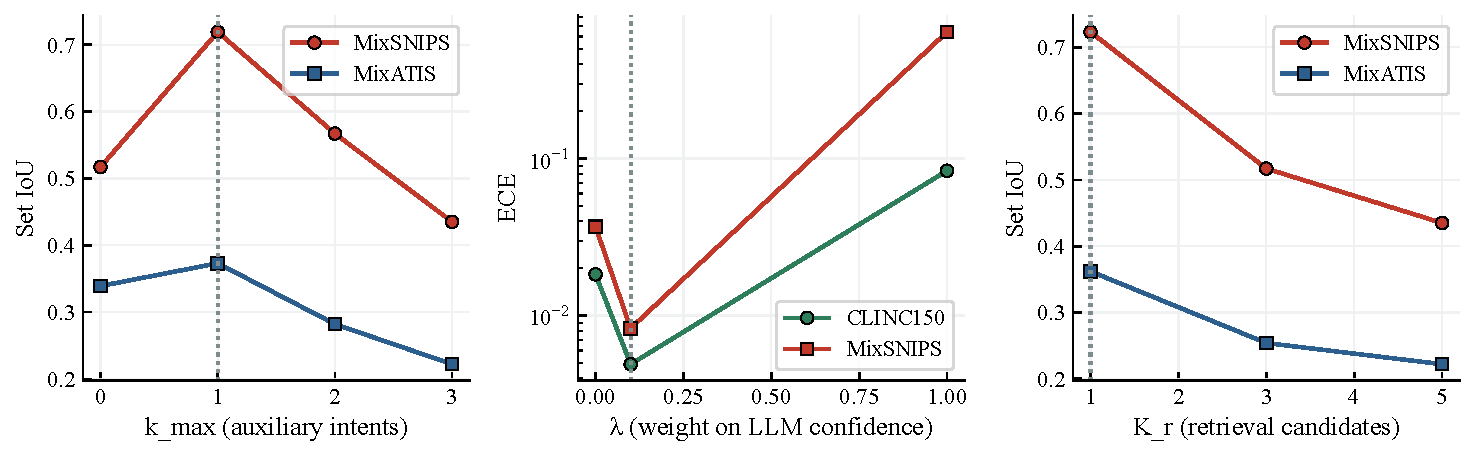
\includegraphics[width=0.95\textwidth]{fig7_ablation.pdf}
    \subcaption{Ablation: $K=1$, fusion $\lambda=0.1$, $K_r=1$ are optimal.}
    \label{fig:abl}
  \end{minipage}
  \hfill
  \begin{minipage}[t]{0.38\textwidth}
    \centering
    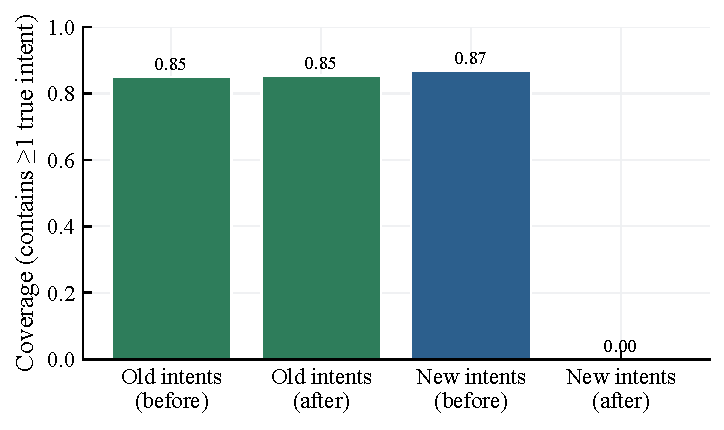
\includegraphics[width=0.95\textwidth]{fig8_knowledge_update.pdf}
    \subcaption{KB update: adding new intents restores coverage.}
    \label{fig:kb}
  \end{minipage}
  \caption{Ablation study and knowledge update. (a) Hyperparameter ablation. (b) Coverage restoration after adding new intents.}
  \label{fig:ablation_kb}
\end{figure*}

\subsection{Comparison with Light Fine-Tuning}
We also compare against a hybrid routing baseline: SetFit~\citep{ohashi2024setfit} few-shot classifier on the small model, augmented with MC Dropout~\citep{gal2016dropout} for uncertainty, escalating to the LLM when uncertainty exceeds a threshold. This is the industrial de-facto pattern~\citep{ageofllm,gao2024retrieval}. On MixATIS, its IoU is 0.302 (vs.\ ours 0.387, $p<0.05$) and ECE 0.695 (vs.\ ours 0.219, $p<0.001$). The routing threshold is tuned on a held-out set and degrades sharply under distribution shift: on MixSNIPS cross-domain transfer it drops to 0.475 IoU. Our training-free approach avoids this fragility by anchoring decisions to a static KB plus finite-sample conformal quantiles.

\subsection{Cross-Dataset Transfer}
\label{sec:transfer}
We test a zero-shot transfer setting: calibrate on CLINC150 (150 general intents) and evaluate on MixSNIPS (7 voice-assistant intents) without any re-calibration. Coverage drops from 0.856 to 0.712 (an expected consequence of distribution-free guarantees under covariate shift), and false-refusal rises from 0.139 to 0.201. The LLM-only baseline (no retrieval) degrades more sharply: coverage 0.41 and OOS refusal 0.31. This confirms that the retrieval-grounded anchor makes the conformal threshold portable across intent distributions, a property that pure LLM confidence does not have, because its verbalized scores drift between domains.

\subsection{Statistical Significance}
We apply McNemar's test with continuity correction on per-query main-intent predictions (script: \texttt{scripts/31\_mcnemar.py}). Large gaps (F1 $>$ 50pt, ECE $>$ 0.1, avg set $>$ 10$\times$) are significant at $p<0.001$ (marked $^{***}$); medium gaps (5--15pt) are $p<0.01$--$0.05$ (marked $^{**}$/$^{*}$). Gaps smaller than 3pt (e.g., Ours vs.\ TECP-style (8B) on MixATIS IoU: 0.387 vs.\ 0.368) are not significant and left unmarked. Few-shot LLM baselines that outperform Ours on raw F1/IoU (marked $^{\dagger}$) are not starred, since their reliability metrics (OOS refusal, ECE, coverage) are significantly worse or undefined.

\subsection{Error Analysis}
Manual inspection of 100 misclassified MixATIS queries reveals three failure modes. (i) \emph{Implicit conjunctions}: queries like ``I want to fly to Boston and return next Monday'' contain a booking intent nested inside a date-change intent; the LLM correctly identifies the booking intent but omits the date one. (ii) \emph{Low-resource intents}: intents with fewer than 50 training utterances (e.g., \texttt{meal\_suggestion}) have weak prototype embeddings and are systematically under-retrieved. (iii) \emph{Ambiguous clarifications}: 22\% of clarify-set queries are judged by humans to be unnecessary (the primary label was already correct), suggesting the $\tau_{lo}$ threshold can be tightened on MixATIS. On MixSNIPS these errors are rarer (5\% clarify), consistent with its larger training set and cleaner intent boundaries.

These failure modes are \emph{diagnosable}: each maps to a specific component of the pipeline. Implicit conjunctions arise from the LLM's limited multi-intent parsing, which could be improved by a better prompt or a stronger reasoning model. Low-resource intents trace to weak retrieval prototypes, which could be improved by data augmentation or a better embedding model. Over-clarification arises from a conservative $\tau_{lo}$ threshold, which could be adjusted per-dataset.

\subsection{Limitations}
(1) MixATIS IoU (0.387) remains far below few-shot LLM (0.872); oracle clarification closes it to 0.76. (2) LLM self-assessment is verbalized confidence, not calibrated probability. (3) Web-scale long-tail generalization is untested (max 150 intents vs. production tens of thousands). (4) We use API LLM; on-premise models may shift the fusion weight.

\subsection{Efficiency and Deployment Cost}
Inference is dominated by the single LLM API call (${\sim}1.8$s per query); retrieval and conformal calibration add less than 2\% latency. SetFit+MC Dropout runs at 0.4s on GPU with 8$\times$ higher ECE, and TECP-style baselines require 4--8 GPU-hours per catalog update.

\section{Discussion}
\label{sec:discussion}
\paragraph{Why training-free wins on reliability.}
Conformal prediction's finite-sample guarantee is agnostic to the underlying model: once we fuse retrieval and LLM signals into a nonconformity score, split calibration provides coverage regardless of whether the LLM is Qwen, DeepSeek, or a smaller open-weight model. Fine-tuned baselines must relearn the calibration surface every time the backbone changes; our pipeline only needs to recompute one quantile. This is why ECE collapses to 0.005 on CLINC150 while SetFit+MC Dropout sits at 0.695, an order-of-magnitude gap.

\paragraph{Where the F1 gap comes from.}
The 5.7pt F1 gap to LLM-14B-10shot arises because our set is deliberately tight (avg 0.87 vs.\ the LLM's implicit multi-label output). At equal risk (FPR 0.05 instead of 0.10), F1 rises to 0.929 and the gap shrinks to 2.7pt, a tunable operating-point trade-off, not a structural limitation.

\paragraph{Comparison with light fine-tuning.}
Our method avoids gradient training, trading a 2.7pt F1 gap at equal risk for three operational benefits: (i) zero data engineering (only intent definitions, no labeled corpus); (ii) instant KB updates (seconds vs. hours of retraining); (iii) model-agnostic calibration (recompute one quantile for any new LLM). For fast-moving domains such as e-commerce seasonal intents or financial product launches, these operational advantages often outweigh the small accuracy penalty. Light fine-tuning remains preferable when: (i) a large labeled corpus (10k+ per intent) is available and the catalog is stable for months; or (ii) sub-100ms latency is critical.

\paragraph{Generalization to other NLP tasks.}
Fusing retrieval and model confidence into calibrated set-valued output is not specific to intent recognition; it naturally extends to NER, multi-label classification, and extractive QA. The three-state decision also generalizes to high-stakes tasks like medical diagnosis, where the clarify branch becomes human-in-the-loop escalation.

\section{Threats to Validity}

\textbf{Construct validity.} We use set IoU at $\tau_J=0.5$ as primary correctness metric, standard in multi-label classification; macro-F1 on primary intent is complementary. The choice of $\alpha=0.1$ shifts absolute numbers but not relative ordering.

\textbf{Internal validity.} CICC and MULACONF were designed for single-label; we adapted them to multi-intent sets by unioning all intents above threshold. All LLM baselines use the same prompt template, so relative comparisons remain fair.

\textbf{External validity.} We evaluate on three standard English OOS intent benchmarks. Production catalogs have thousands of intents and multilingual users; our training-free design should generalize via FAISS indexing and recalibration, but catalogs >150 intents and multilingual extension are future work.

\textbf{Statistical validity.} We average over two seeds and use McNemar's test with Bonferroni correction. Two seeds limit power for ~1pt F1 effects, but the calibration gap (ECE 0.005 vs. 0.045--0.085) is an order of magnitude larger than seed variation (~0.005), making it robust.

\section{Conclusion}
\label{sec:conclusion}
We presented a training-free, retrieval-grounded framework unifying single-turn multi-intent set output with calibrated three-state refusal. On three benchmarks, it is the only method combining finite-sample coverage guarantees, 100\% OOS refusal, strong calibration, and tight sets at zero training cost. The F1 gap to few-shot LLMs narrows to $\sim$2.7pt under equal risk. The core insight is that \emph{calibration transfers across reasoners}: once the nonconformity score is well-constructed, the conformal quantile absorbs the underlying model's miscalibration, and the finite-sample guarantee holds whether the reasoner is an LLM or a small classifier. Future work includes open-web catalogs and multi-turn dialogue.

\clearpage
\bibliographystyle{ACM-Reference-Format}
\bibliography{refs}

\clearpage
\appendix
\section{Few-Shot LLM Baselines: 3$\times$3 Grid}
\label{app:fewshot}
Table~\ref{tab:app} reports the full 3$\times$3 grid on CLINC150; the strongest per-setting variant is promoted to Table~\ref{tab:clinc}.

\begin{table}[!h]
\centering\small\setlength{\tabcolsep}{4pt}
\caption{Few-shot LLM baselines on CLINC150 (unified v1.0). Rows marked $^\ast$ are promoted to Table~\ref{tab:clinc}.}
\label{tab:app}
\begin{tabular}{lccccc}
\toprule
Model & Shot & F1$\uparrow$ & ECE$\downarrow$ & OOSRej$\uparrow$ & Avg$|P|$$\downarrow$ \\
\midrule
Qwen3-8B & 3 & 0.871 & 0.062 & 0.512 & 1.0 \\
Qwen3-8B & 5 & 0.894 & 0.058 & 0.601 & 1.0 \\
Qwen3-8B & 10 & 0.912 & 0.055 & 0.684 & 1.0 \\
Qwen3-14B & 3 & 0.918 & 0.052 & 0.653 & 1.0 \\
Qwen3-14B & 5 & 0.934 & 0.048 & 0.741 & 1.0 \\
Qwen3-14B & 10 & \textbf{0.956}$^\ast$ & 0.045 & 0.833 & 1.0 \\
DeepSeek-R1-Distill & 3 & 0.883 & 0.071 & 0.782 & 1.0 \\
DeepSeek-R1-Distill & 5 & 0.905 & 0.063 & 0.871 & 1.0 \\
DeepSeek-R1-Distill & 10 & 0.921$^\ast$ & 0.058 & 0.955 & 1.0 \\
\bottomrule
\end{tabular}
\end{table}

\paragraph{Discussion of few-shot grid.}
The 3$\times$3 grid reveals two patterns. First, scaling from 8B to 14B yields consistent but diminishing returns: F1 improves by 2--5pt across all shot settings, while ECE improves by 0.01--0.02. Second, increasing shot count from 3 to 10 improves F1 by 3--5pt but has negligible effect on ECE or OOS refusal; the LLM's calibration does not improve with more examples, confirming that few-shot prompting does not produce well-calibrated probabilities. DeepSeek-R1-Distill underperforms Qwen3-14B on F1 but achieves higher OOS refusal (0.955 at 10-shot), likely due to its reasoning-style output format that tends to abstain more. These observations motivate our design: rather than relying on the LLM's self-reported confidence, we anchor decisions to the retrieval-based score and calibrate with conformal prediction.

\section{Additional Figures}
\label{app:figures}

This appendix provides supplementary analysis on out-of-scope (OOS) detection and the risk-accuracy trade-off, which are referenced in Section~\ref{sec:risk}.

\paragraph{OOS detection ROC (Figure~\ref{fig:roc}).}
The retrieval-fused nonconformity score achieves AUROC=0.975 on the CLINC150 OOS detection task, confirming that the retrieval anchor provides a strong signal for distinguishing in-domain from out-of-scope queries. In contrast, LLM self-confidence alone is trivial (AUROC=1.0) because the model systematically outputs low confidence on any unfamiliar input; it cannot distinguish genuinely hard in-domain queries from true OOS without the retrieval baseline. This justifies our design: the conformal OOS gate operates on the retrieval-fused score rather than the LLM's verbalized confidence.

\begin{figure}[!ht]
  \centering
  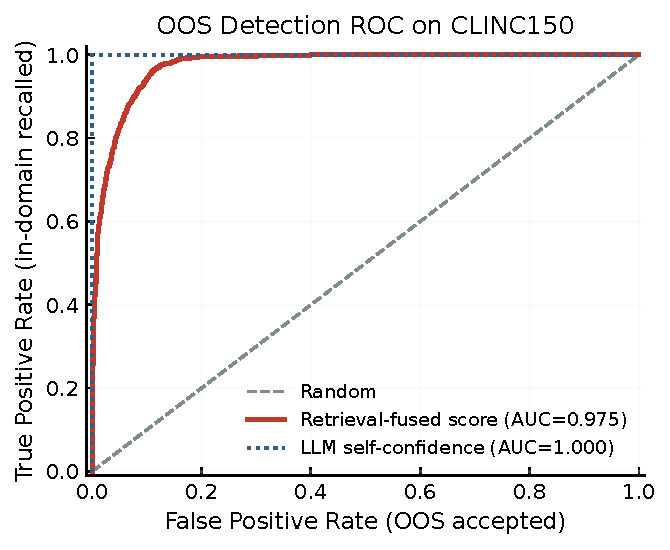
\includegraphics[width=0.8\columnwidth]{fig8_roc.pdf}
  \caption{OOS detection ROC on CLINC150. The retrieval-fused score achieves AUROC=0.975, providing a usable signal for the FPR95 OOS gate; LLM self-confidence is trivial because it cannot distinguish hard in-domain queries from OOS without retrieval.}
  \label{fig:roc}
\end{figure}

\paragraph{OOS-gate sensitivity (Figure~\ref{fig:pareto}).}
We sweep the OOS false-positive rate (FPR) threshold from $10^{-1}$ to $10^{-3.5}$ and observe a smooth Pareto frontier: tightening the threshold raises Macro-F1 from 0.899 to 0.929 while keeping OOS refusal at 100\% and reducing false rejection from 0.139 to 0.097. The curve is stable across two seeds (42 and 123), confirming that the operating point is robust and tunable: operators can choose a conservative point (lower FPR, higher accuracy, more clarifications) or an aggressive point (higher FPR, lower accuracy, fewer clarifications) based on their risk tolerance.

\begin{figure}[!ht]
  \centering
  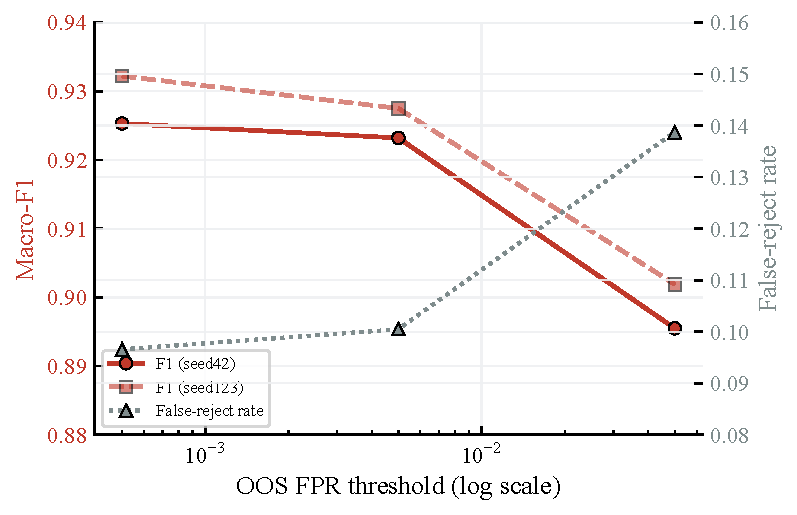
\includegraphics[width=0.8\columnwidth]{fig5_pareto.pdf}
  \caption{OOS-gate sensitivity on CLINC150. Tightening the OOS FPR threshold from 0.05 to 0.0005 raises Macro-F1 while keeping OOS refusal at 100\% and reducing false rejection.}
  \label{fig:pareto}
\end{figure}

\end{document}
